\section{Introduction}


CBMC is being used by at AWS to verify memory safety and functional
correctness of foundational C libraries such as AWS C Common and AWS
Encryption SDK. It is a robust tool that can handle almost all of C
constructs seen in practice, and finds bugs that are very hard to find
by unit/integration testing. Moreover, CBMC is easy enough to deploy
that many developers use it routinely at AWS. But most of the current
proofs are bounded in the size of the inputs they can handle. For
instance, current proof of \emph{aws\_rray\_eq} program (shown below)
assumes a bound of size 20 on the input arrays.

\begin{figure}[H]
  \centering
  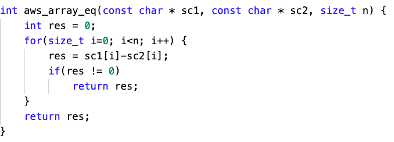
\includegraphics[scale=0.6]{Picture1.png}
  \caption{Arrays equals program}
\end{figure}

The reason is CBMC has to first unwind the ‘for’ loop a small number
of times, here 20, to obtain a straight-line code which can then be
translated into a SAT problem. Since the loop is used to traverse the
array, limiting the number of unwindings is in effect the same as
ignoring entries at indices greater than 20. For instance, the bug in
the following modified \emph{aws\_array\_eq} program will not be found by
unwinding the loop fewer than 100 times.

\begin{figure}[H]
  \centering
  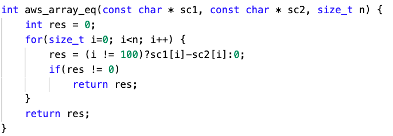
\includegraphics[scale=0.6]{Picture2.png}
  \caption{Buggy version}
\end{figure}

\nop{
We describe an abstraction technique that in conjunction with CBMC
allows us to write unbounded proofs of C programs with minimal user
effort. The key insight in our method is that by reducing replication in
the data structures in C programs we reduce the number of loop
unrollings required. Once this reduction is performed CBMC is then
able to give unbounded proofs for programs.}

This is an instance of a more general problem that is also seen in
hardware (HW) and protocol verification. HW designs have large
memories, register banks, buffers and such that exhibit a high degree
of replication. Data Type Reduction, studied by Long~\cite{long},
McMillan~\cite{mcmillan}, Wolpert~\cite{wolpert} and others, has been
successfully used to tackle this problem. The idea simply is that a
large, potentially unbounded data type can be replaced by a small
finite abstract data type that tracks specific values precisely and
the rest are replaced by abstract values. For example, a set of
indices [1..n] can be replaced by an abstract type [{\tt i},\(\bot\)]
which tracks a particular index {\tt i} precisely and the rest of the
indices imprecisely. This abstraction retains enough information to
decide value of terms like \({\tt i} \neq {\tt j}\) and {\tt a[i]}
precisely but not those of terms like \({\tt j} \neq {\tt k}\) and
{\tt a[k]} where {\tt j,k} are different from {\tt i}.

In case of distributed protocols like cache coherence protocols there
is replication in the form of multiple identical cache agents running
in different processes.  Replication reducing techniques such as the CMP
technique~\cite{self} have been used to scale model checkers to any
required bound size.

\nop{For example, in HW verification Data Type Reduction has been highly
successful. It is a special case of Abstraction Interpretation~\cite{abstint},
that has been studied by multiple works such as
Wolpert~\cite{wolpert}, Long~\cite{long}, McMillan~\cite{mcmillan} and
others. The idea simply is that a large, potentially unbounded data
type can be replaced by a small finite abstract data type that tracks
specific values precisely and the rest are replaced by abstract
values. For example, a set of indices [1..n] can be replaced by an
abstract type [{\tt i},\(\bot\)] which tracks a particular index {\tt i} precisely and
the rest of the indices imprecisely. This abstraction retains enough
information to decide value of terms like \({\tt i} \neq {\tt j}\) and {\tt a[i]} precisely but
not those of terms like \({\tt j} \neq {\tt k}\) and {\tt a[k]} where {\tt j,k} are different from {\tt i}.}

We can use a similar abstractions to reduce replication and help CBMC
scale to any required input size. Consider the \emph{aws\_array\_eq}
program again which compares two arrays by iterating over them. In
each iteration it compares {\tt sc1[i]} against {\tt sc2[i]} and
entries at different indices don’t interfere with one another. A bug
in this program will be localized to one particular index and what
happens at the other indices can be ignored.

If we can guess the precise location ‘c’ at which {\tt sc1} and {\tt
  sc2} differ we could have collapsed all the entries before ‘c’ into
one location and all the entries after ‘c’ into another
location. Reduced {\tt sc1} and {\tt sc2} arrays with just 3 indices
would still be sufficient to expose the bug in the program.

Because we don’t know the value of ‘c’ upfront, we introduce it as a
free variable and abstract the arrays {\tt sc1}, {\tt sc2} with
respect to it \emph{dynamically}. When we run CBMC it will try all
possible values for ‘c’ and for each value of ‘c’ the abstracted
arrays are of length only 3. If there is a bug in the original program
it will be found in the abstract program too. If the abstract program
has no bug then we can conclude that the original program is bug free
as well. Intuitively, the original program has a deep state space
whereas the abstract program has broad but shallow state space. CBMC
can completely explore the latter but not the former.

We call this abstraction Replication Reducing Abstraction or RRA for
short. We applied this technique to a collection of AWS C Common
examples that currently have bounded proofs using CBMC. These examples
are daunting enough that most of the tools in SVComp 2020 failed to
handle them in an unbounded fashion. We had to make slight
modification to the default {\tt memcpy} and {\tt memcmp} functions as
they use pointer arithmetic to traverse/access array contents. We
rewrote these to use clean array indexing instead as the current
version of RRA doesn't yet handle full pointer arithmetic.

We will next describe a minimal program model without pointer
arithmetic and use it to formally define how RRA transforms a
program. The section after that goes over the soundness of the
abstraction. Apart from soundness another concern when doing
abstraction is to eliminate or reduce spurious counterexamples. We
describe a simple transformation for properties that is quite
useful in reducing spurious failures. We end the paper by going over
the examples we have handled and surveying the related work.
